% Complex numbers on slanted graph paper
% Mostafa Derraz, 2026. Short version of "General Numbers: The Number Plane
% Beyond the Right Angle" (Zenodo, doi:10.5281/zenodo.24091305), prepared as an
% Article for The Mathematical Gazette. The full version is left unchanged.
\documentclass[11pt,a4paper]{article}

\usepackage[T1]{fontenc}
\usepackage{lmodern}
\usepackage[sc,osf]{mathpazo}
\linespread{1.05}
\usepackage[a4paper,margin=3cm]{geometry}
\usepackage{microtype}
\usepackage{amsmath,amssymb,amsthm,mathtools}
\usepackage{tikz}
\usetikzlibrary{arrows.meta,calc,angles,quotes}
\usepackage{enumitem}
\usepackage{booktabs,array}
\usepackage[hidelinks]{hyperref}
\usepackage[capitalise,nameinlink,noabbrev]{cleveref}

\theoremstyle{plain}
\newtheorem{theorem}{Theorem}
\newtheorem{proposition}[theorem]{Proposition}
\newtheorem{corollary}[theorem]{Corollary}
\theoremstyle{definition}
\newtheorem{definition}[theorem]{Definition}

\newcommand{\pb}{\bar{\phi}}                     % angle of the Composer axis
\newcommand{\Gp}{\mathcal{G}_{\bar{\phi}}}       % Composer Unit
\newcommand{\up}{\vec{u}_{\bar{\phi}}}           % direction of the Composer Unit
\newcommand{\Jp}{\mathcal{J}_{\bar{\phi}}}       % Turning Unit
\newcommand{\GNp}{\mathbb{G}_{\bar{\phi}}}       % relative plane
\newcommand{\C}{\mathbb{C}}
\newcommand{\R}{\mathbb{R}}
\newcommand{\G}{\lvert\Gp\rvert}                 % length of the Composer Unit
\renewcommand{\Re}{\operatorname{Re}}
\DeclareMathOperator{\Com}{Com}
\DeclareMathOperator{\Sh}{Sh}
\DeclareMathOperator{\Ht}{Ht}

\setlist[enumerate]{leftmargin=*,itemsep=2pt}
\raggedbottom

\title{Complex numbers on slanted graph paper}
\author{Mostafa Derraz\\[2pt]
\small Independent scholar, Tangier, Morocco\\
\small e-mail: \texttt{m.derraz@proton.me}\quad ORCID: \texttt{0000-0002-2307-9298}}
\date{}

\begin{document}
\maketitle

\begin{abstract}
\noindent Everyone draws the complex plane on square graph paper, with the imaginary axis upright and a unit of length one. Here I redraw it on slanted paper, where the second axis leans at an angle and its unit has a length of its own. The numbers stay the same, and so does Wessel's rule for multiplying them. Many familiar laws do not survive. The square of the leaning unit is no longer $-1$. The conjugate moves the real part. The Composer part of a product is built from the shadows of the factors, and a part of a number can even be longer than the number. Each of these laws has a general form, in which the shadow and the height of a number take over the work of its real and imaginary parts, and the coordinates of the unit circle become the sine and cosine of an oblique triangle. Slanted paper therefore sorts what we know about complex numbers into two piles, facts about the numbers and facts about the square paper. The article closes with five short exercises on isometric paper that ask students to tell the two apart.
\end{abstract}

\noindent\textbf{Keywords:} complex numbers; oblique coordinates; conjugate; Euler's formula; generalized complex numbers

%====================================================================
\section{The quarter turn}
%====================================================================

In 1797 the Norwegian-born surveyor Caspar Wessel showed the Royal Danish Academy how to calculate with directions \cite{Wessel}. Give an arrow by its length and its angle, he said, and the rule \emph{multiply the lengths and add the angles} behaves exactly like a multiplication. Multiplying by $i$ is then a quarter turn about $0$. Read this way, $i^2 = -1$ says no more than that two quarter turns make a half turn. Argand found the same picture in 1806 \cite{Argand}, and in 1837 Hamilton rebuilt it as an algebra of pairs of real numbers \cite{Hamilton}.

The picture carries a habit so familiar that nobody states it. We draw it on square graph paper. The imaginary axis stands at a right angle to the real one, and its unit is one long. I want to ask what happens to complex arithmetic if we keep the arrows and Wessel's rule and change only the paper, to a \emph{slanted} sheet whose second family of lines leans at an angle $\pb$ and whose second unit has a length of its own (\cref{fig:graph-paper}).

Nothing happens to the numbers, and I would rather say so at once. The arrows on the page and their products stay where they were, and only their names change. The \emph{laws} are another matter. Take $z + \bar z = 2\Re z$, or $\Re\bar z = \Re z$. Every student learns these, and both hold only because the paper is square. On slanted paper they fail and something else takes their place, which is easy to find with school algebra and trigonometry. In finding it we learn which facts about $\C$ belong to the numbers and which belong to the paper. I think that difference is worth teaching, and \cref{sec:classroom} has exercises for students who have just met complex numbers.

\begin{figure}[tb]
\centering
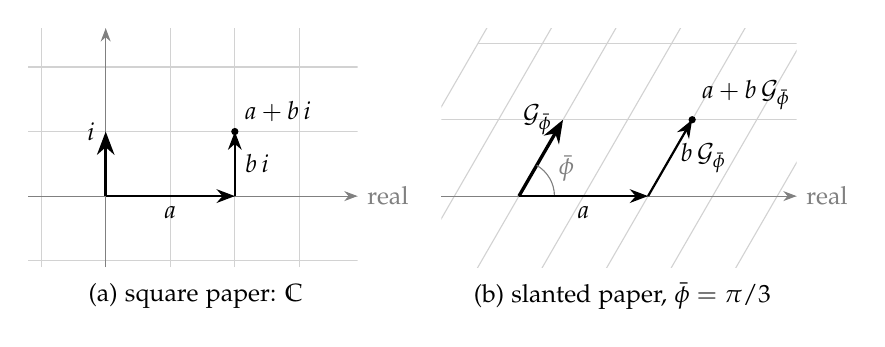
\begin{tikzpicture}[>=Stealth, scale=0.82, every node/.style={font=\small}]
  % ---------- (a) square paper ----------
  \begin{scope}
    \clip (-1.2,-1.1) rectangle (3.9,2.6);
    \foreach \a in {-1,...,4} \draw[gray!35] (\a,-1.1) -- (\a,2.6);
    \foreach \b in {-1,...,3} \draw[gray!35] (-1.2,\b) -- (3.9,\b);
  \end{scope}
  \draw[->, gray] (-1.2,0) -- (3.9,0) node[right] {real};
  \draw[->, gray] (0,-1.1) -- (0,2.6);
  \draw[->, very thick] (0,0) -- (0,1) node[left] {$i$};
  \draw[->, thick] (0,0) -- (2,0) node[below, pos=0.5] {$a$};
  \draw[->, thick] (2,0) -- (2,1) node[right, pos=0.5] {$b\,i$};
  \fill (2,1) circle (1.6pt) node[above right] {$a + b\,i$};
  \node at (1.4,-1.55) {(a) square paper: $\C$};
  % ---------- (b) slanted paper ----------
  \begin{scope}[xshift=6.4cm]
    \pgfmathsetmacro{\gx}{1.366*cos(60)}
    \pgfmathsetmacro{\gy}{1.366*sin(60)}
    \begin{scope}
      \clip (-1.2,-1.1) rectangle (4.3,2.6);
      \foreach \a in {-3,...,5} \draw[gray!35] ($(\a,0)+(-2*\gx,-2*\gy)$) -- ($(\a,0)+(3*\gx,3*\gy)$);
      \foreach \b in {-1,...,2} \draw[gray!35] ($(-2,0)+(\b*\gx,\b*\gy)$) -- ($(5,0)+(\b*\gx,\b*\gy)$);
    \end{scope}
    \draw[->, gray] (-1.2,0) -- (4.3,0) node[right] {real};
    \draw[->, very thick] (0,0) -- (\gx,\gy) node[left] {$\mathcal{G}_{\bar{\phi}}$};
    \draw[gray] (0.55,0) arc (0:60:0.55);
    \node[gray] at (30:0.85) {$\bar{\phi}$};
    \draw[->, thick] (0,0) -- (2,0) node[below, pos=0.5] {$a$};
    \draw[->, thick] (2,0) -- ($(2,0)+(\gx,\gy)$) node[right, pos=0.5] {$b\,\mathcal{G}_{\bar{\phi}}$};
    \fill ($(2,0)+(\gx,\gy)$) circle (1.6pt) node[above right] {$a + b\,\mathcal{G}_{\bar{\phi}}$};
    \node at (1.6,-1.55) {(b) slanted paper, $\bar{\phi} = \pi/3$};
  \end{scope}
\end{tikzpicture}
\caption{Square and slanted graph paper, with $a = 2$ and $b = 1$. (a) The number $a + bi$ is $a$ steps along the real axis and $b$ steps of length one straight up. (b) The number $a + b\,\Gp$ is $a$ steps along the real axis and $b$ steps of the leaning unit $\Gp$, here of length $\cos\frac{\pi}{3} + \sin\frac{\pi}{3} \approx 1.366$.}
\label{fig:graph-paper}
\end{figure}

%====================================================================
\section{Slanted paper}
%====================================================================

Identify the page with $\C$ in the usual way. Choose an angle $\pb$ with $0 < \pb < \pi$ and a positive length $\G$, and let
\[
\up = e^{i\pb} , \qquad \Gp = \G\,\up .
\]
I call $\Gp$ the \emph{Composer Unit} and the line through it the \emph{Composer axis}. Since $\Gp$ is not a real multiple of $1$, every arrow $z$ of the page can be written in exactly one way as
\[
z = a + b\,\Gp , \qquad a, b \in \R ,
\]
so $a$ steps along the real axis and then $b$ steps of the Composer Unit. I call $a$ the \emph{real part} of $z$, written $\Re z$, and $b\,\Gp$ its \emph{Composer part}, $\Com z$. Named like this, added part by part and multiplied by Wessel's rule, the arrows make up what I call the \emph{relative plane} $\GNp$. With its two operations it is just $\C$. Only the frame $\{1, \Gp\}$ is new.

An arrow also keeps the two readings it had on square paper. Its \emph{shadow} $\Sh z$ is the signed length of its perpendicular projection on the real axis. Its \emph{height} $\Ht z$ is the signed distance of its tip above that axis. From the picture,
\begin{equation}\label{eq:shadow-height}
\Sh z = a + b\,\G\cos\pb , \qquad \Ht z = b\,\G\sin\pb .
\end{equation}
On square paper $\pb = \pi/2$ and $\G = 1$, and the shadow and height are just the real and imaginary parts. Lean the axis and the two pairs come apart. Almost everything in this article is about the gap between them.

\paragraph{A choice of length.} Apart from the numbers in the example of \cref{sec:example}, nothing below depends on how $\G$ is chosen. I use one choice that ties the length to the angle. The unit is made as long as the two shadows of its direction on the axes of the page, added together,
\begin{equation}\label{eq:axiom}
\G = \lvert\cos\pb + \sin\pb\rvert = \sqrt{2}\,\Bigl\lvert\sin\Bigl(\pb + \frac{\pi}{4}\Bigr)\Bigr\rvert .
\end{equation}
At $\pb = \pi/2$ this gives $\G = 1$ and $\Gp = i$, so square paper belongs to the family. The length climbs to $\sqrt{2}$ at $\pi/4$ and drops to $0$ at $3\pi/4$, where the paper collapses (\cref{fig:fan}). A length $A$ between $1$ and $\sqrt{2}$ belongs to exactly two angles, mirror images in the line at $\pi/4$. Because $A^2 = (\cos\pb + \sin\pb)^2 = 1 + \sin 2\pb$, they are
\[
\pb_1 = \tfrac{1}{2}\arcsin(A^2 - 1) , \qquad \pb_2 = \tfrac{\pi}{2} - \pb_1 .
\]
The length $1.16043$, which I use later, gives $10.14^\circ$ and $79.86^\circ$.

\begin{figure}[tb]
\centering
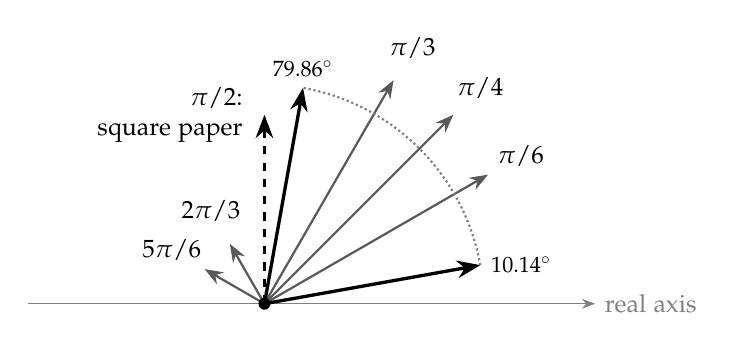
\begin{tikzpicture}[>=Stealth, scale=2.4, every node/.style={font=\small}]
  \draw[->, gray] (-1.25,0) -- (1.75,0) node[right] {real axis};
  \foreach \ang/\len/\lab in {30/1.366/{\pi/6}, 45/1.414/{\pi/4}, 60/1.366/{\pi/3}, 120/0.366/{2\pi/3}, 150/0.366/{5\pi/6}}
  {
    \draw[->, thick, gray!70!black] (0,0) -- (\ang:\len);
    \node at (\ang:{\len+0.2}) {$\lab$};
  }
  \draw[gray, densely dotted, thick] (10.14:1.16043) arc (10.14:79.86:1.16043);
  \draw[->, very thick] (0,0) -- (10.14:1.16043) node[right, font=\footnotesize] {$10.14^\circ$};
  \draw[->, very thick] (0,0) -- (79.86:1.16043) node[above, font=\footnotesize] {$79.86^\circ$};
  \draw[->, very thick, dashed] (0,0) -- (90:1) node[left=4pt, align=right] {$\pi/2$:\\ square paper};
  \fill (0,0) circle (0.9pt);
\end{tikzpicture}
\caption{A fan of Composer Units with the length \eqref{eq:axiom}. Each arrow is drawn at its angle $\pb$ with the length $\lvert\cos\pb + \sin\pb\rvert$; the dashed arrow is $i$. The two thick arrows have the same length, $1.16043$, and the dotted arc joins them.}
\label{fig:fan}
\end{figure}

%====================================================================
\section{Arithmetic on slanted paper}
%====================================================================

Throughout, $z = a + b\,\Gp$ and $w = c + d\,\Gp$.

\paragraph{The square of the unit.} The multiplication table of square paper has a single entry, $i^2 = -1$. Slanted paper needs a different one.

\begin{proposition}[The Rule of the Square]\label{prop:square}
$\up^2 = 2\cos\pb\;\up - 1$, and so
\[
\Gp^2 = 2\G\cos\pb\;\Gp - \G^2 .
\]
\end{proposition}

\begin{proof}
$e^{i\pb}$ is a root of $t^2 - 2\cos\pb\,t + 1 = (t - e^{i\pb})(t - e^{-i\pb})$. Multiply by $\G^2$.
\end{proof}

Put $\pb = \pi/2$ and the rule becomes $i^2 = -1$. At any other angle the square of the unit has a real part \emph{and} a Composer part, so it points along the real axis only on square paper.

\paragraph{The product.} Multiply out $(a + b\,\Gp)(c + d\,\Gp)$ and use the Rule of the Square:
\begin{equation}\label{eq:product}
zw = \bigl(ac - \G^2\,bd\bigr) + \bigl(ad + bc + 2\G\cos\pb\;bd\bigr)\,\Gp .
\end{equation}
I find two things in this formula worth a second look. The angle enters the real part $ac - \G^2bd$ only through the length of the unit, so the two angles that share a length share this formula too. The Composer coordinate regroups as $(a + b\G\cos\pb)\,d + (c + d\G\cos\pb)\,b$, and by \eqref{eq:shadow-height} that is
\begin{equation}\label{eq:com-product}
\Com(zw) = \Sh(z)\,\Com(w) + \Sh(w)\,\Com(z) .
\end{equation}
On square paper this is the familiar $\operatorname{Im}(zw) = \Re z\operatorname{Im} w + \Re w\operatorname{Im} z$. On slanted paper the \emph{shadows} of the factors turn up in the places where the real parts used to be.

\paragraph{The conjugate.} The paper cannot change what the conjugate $\bar z$ is. It is still the mirror image of $z$ in the real axis. The question is what to call it. The mirror image of $\up = e^{i\pb}$ is $e^{-i\pb} = 2\cos\pb - \up$, so the mirror image of $a + b\,\G\up$ is
\begin{equation}\label{eq:conjugate}
\bar z = \bigl(a + 2b\,\G\cos\pb\bigr) - b\,\Gp .
\end{equation}
The Composer part is reversed, as you would expect. The surprise is that the \emph{real part moves}. The number habit makes us write, $a - b\,\Gp$, is another arrow altogether. I call it the \emph{skew flip} of $z$. It reflects $z$ in the real axis, but along the Composer axis, where the conjugate reflects straight down. The skew flip keeps the real part and changes the length, and
\[
(a + b\,\Gp)(a - b\,\Gp) = a^2 + b^2\G^2 - 2b^2\G\cos\pb\;\Gp
\]
is not even real unless $b = 0$. So each of the two keeps one property and loses the other. The conjugate holds on to the length, the skew flip to the real part, and only on square paper do they agree.

Putting \eqref{eq:conjugate} beside \eqref{eq:shadow-height},
\[
z + \bar z = 2\Sh z , \qquad \Re\bar z = 2\Sh z - \Re z ,
\]
and the shadow of $z$ sits halfway between the real parts of $z$ and $\bar z$. Multiplying $z$ by $\bar z$ with \eqref{eq:product} gives the squared length,
\begin{equation}\label{eq:norm}
z\bar z = \lvert z\rvert^2 = a^2 + 2ab\,\G\cos\pb + b^2\G^2 ,
\end{equation}
which is just the law of cosines in the triangle made by the two steps of $z$. Lengths multiply under Wessel's rule, so \eqref{eq:norm} is a \emph{multiplicative} quadratic form. With $zw = s + t\,\Gp$,
\[
\bigl(a^2 + 2ab\G\cos\pb + b^2\G^2\bigr)\bigl(c^2 + 2cd\G\cos\pb + d^2\G^2\bigr) = s^2 + 2st\G\cos\pb + t^2\G^2 .
\]
At $\pb = \pi/2$ and $\G = 1$ this is the old two-square identity of Brahmagupta and Fibonacci. Division works as it always does, $1/z = \bar z/\lvert z\rvert^2$.

\paragraph{The Turning Unit.} On slanted paper $\Gp^2 \neq -1$. Still, some arrow on the page squares to $-1$, namely $i$, one unit straight up. In the slanted frame it is
\begin{equation}\label{eq:turning}
\Jp = \frac{\up - \cos\pb}{\sin\pb} = -\cot\pb + \frac{\Gp}{\G\sin\pb} ,
\end{equation}
and I call it the \emph{Turning Unit}. Multiplying by $\Jp$ is the quarter turn, $\Jp^2 = -1$, and every number is its shadow plus its height times the Turning Unit,
\[
z = \Sh z + \Ht z\;\Jp .
\]
That equation is the way back to square paper. The map $z \mapsto \Sh z + i\,\Ht z$ is an isomorphism of fields from $\GNp$ onto $\C$, sending $\Gp$ to $\G\,e^{i\pb}$ and $\Jp$ to $i$.

Readers who know hypercomplex numbers will have recognised the algebra by now. The Rule of the Square has the form $\Gp^2 = p + q\,\Gp$, with $p = -\G^2$ and $q = 2\G\cos\pb$, and $q^2 + 4p = -4\G^2\sin^2\pb$ is negative. So the relative planes are the \emph{elliptic generalized complex numbers} \cite{HarkinHarkin, KantorSolodovnikov, Yaglom}, here drawn as a picture, and \eqref{eq:turning} is the standard element that reduces the elliptic case to $\C$. It works the other way round as well. Any elliptic pair $(p, q)$ is a slanted paper, with the length $\sqrt{-p}$ and the angle $\arccos\bigl(q/(2\sqrt{-p})\bigr)$.

%====================================================================
\section{Habits that fail}
%====================================================================

Now copy the laws of $\C$ onto slanted paper without thinking, writing $\Gp$ for $i$ and the Composer coordinate $b$ for the imaginary part. \Cref{tab:habits} lists what goes wrong. Each habit in the left column breaks as soon as $\cos\pb \neq 0$. Each law in the right column holds on every slanted paper, and at $\pb = \pi/2$, $\G = 1$ it turns back into the habit beside it.

\begin{table}[tb]
\centering
\small
\renewcommand{\arraystretch}{1.3}
\begin{tabular}{@{}l l@{}}
\toprule
\textbf{a habit of square paper} & \textbf{the law on slanted paper} \\
\midrule
$i^2 = -1$ & $\Gp^2 = 2\G\cos\pb\;\Gp - \G^2$; it is $\Jp$ that squares to $-1$ \\
$\Re\bar z = \Re z$ & $\Re\bar z = 2\Sh z - \Re z$ \\
$z + \bar z = 2\Re z$ & $z + \bar z = 2\Sh z$ \\
$z\bar z = (\Re z)^2 + (\operatorname{Im} z)^2$ & $z\bar z = a^2 + 2ab\,\G\cos\pb + b^2\G^2 = (\Sh z)^2 + (\Ht z)^2$ \\
$(a + bi)(a - bi)$ is real & $(a + b\,\Gp)(a - b\,\Gp)$ has the Composer part $-2b^2\G\cos\pb\;\Gp$ \\
$\operatorname{Im}(zw) = \Re z\operatorname{Im} w + \Re w\operatorname{Im} z$ & $\Com(zw) = \Sh z\,\Com w + \Sh w\,\Com z$ \\
$\lvert\Re z\rvert \le \lvert z\rvert$ & $\lvert\Re z\rvert \le \lvert z\rvert/\sin\pb$, and the bound is reached \\
$e^{i\theta} = \cos\theta + i\sin\theta$ & $e^{\theta\Jp} = \cos(\theta, \pb - \theta) + \sin(\theta, \pb - \theta)\,\up$ \\
\bottomrule
\end{tabular}
\caption{Habits of square paper and the laws that replace them on slanted paper, with $z = a + b\,\Gp$. The last line is explained in \cref{sec:trig}.}
\label{tab:habits}
\end{table}

The seventh line is the one that surprises. On square paper no part of a number is longer than the number. On slanted paper a part can be. Take the Turning Unit, of length $1$. By \eqref{eq:turning} its Composer part, $\Gp/(\G\sin\pb)$, is $1/\sin\pb > 1$ long, and its real part is $-\cot\pb$, so the walk along the two leaning steps overshoots and then comes back. In general the sine rule in the triangle of the two steps bounds both parts by $\lvert z\rvert/\sin\pb$. The readings never overshoot: $\lvert\Sh z\rvert \le \lvert z\rvert$ and $\lvert\Ht z\rvert \le \lvert z\rvert$.

Look down the left column of the table, first six lines. Every one of those laws is about the \emph{frame}. Each uses the real and imaginary parts, and each comes through to slanted paper only once the parts are swapped for the shadow and the height. Then there are the facts that never needed swapping, like $\lvert zw\rvert = \lvert z\rvert\,\lvert w\rvert$, or that conjugation is the mirror image. Those are about the \emph{arrows}.

%====================================================================
\section{The trigonometry of slanted paper}\label{sec:trig}
%====================================================================

On square paper the unit arrow at the angle $\theta$ has the coordinates $\cos\theta$ and $\sin\theta$. Slant the paper and the coordinates become the sides of an oblique triangle. They still have a closed form.

Write the unit arrow $e^{i\theta}$ as $x + y\,\up$. The imaginary parts give $\sin\theta = y\sin\pb$, and the real parts give $\cos\theta = x + y\cos\pb$. So
\begin{equation}\label{eq:gs}
x = \frac{\sin(\pb - \theta)}{\sin\pb} , \qquad y = \frac{\sin\theta}{\sin\pb} .
\end{equation}
These are the sides of the triangle with vertices $0$, $x$ and $e^{i\theta}$, read off by the law of sines. Its angles are $\theta$ at $0$, $\phi = \pb - \theta$ at $e^{i\theta}$, and $\pi - \pb$ at $x$. I studied these ratios in an earlier paper \cite{DerrazGSP} as functions of two angles, the \emph{general sine and cosine}
\[
\sin(\alpha, \phi) = \frac{\sin\alpha}{\sin(\alpha + \phi)} , \qquad \cos(\alpha, \phi) = \frac{\sin\phi}{\sin(\alpha + \phi)} ,
\]
which reduce to the classical functions when $\alpha + \phi = \pi/2$. Put $\alpha = \theta$ and $\phi = \pb - \theta$, and \eqref{eq:gs} says that the general cosine and sine are the coordinates of the unit circle in the slanted frame. I shorten them to
\[
C_\theta = \cos(\theta, \pb - \theta) = \frac{\sin(\pb - \theta)}{\sin\pb} , \qquad S_\theta = \sin(\theta, \pb - \theta) = \frac{\sin\theta}{\sin\pb} .
\]
Any $z \neq 0$ at the angle $\alpha$ is then $z = \lvert z\rvert\,(C_\alpha + S_\alpha\,\up)$, which is the polar form of the slanted frame. For a unit arrow, \eqref{eq:norm} turns into Pythagoras with a cross term,
\[
C_\theta^2 + 2\cos\pb\;C_\theta S_\theta + S_\theta^2 = 1 .
\]

\paragraph{Multiplying means turning.} Wessel's rule says the unit arrows at $\alpha$ and $\beta$ multiply to the unit arrow at $\alpha + \beta$. Expand $(C_\alpha + S_\alpha\up)(C_\beta + S_\beta\up)$ with the Rule of the Square, compare parts, and out come the \emph{addition formulas of slanted paper},
\[
C_{\alpha + \beta} = C_\alpha C_\beta - S_\alpha S_\beta , \qquad S_{\alpha + \beta} = C_\alpha S_\beta + S_\alpha C_\beta + 2\cos\pb\;S_\alpha S_\beta .
\]
At $\pb = \pi/2$ these are the usual addition formulas. A student who distrusts the argument can check both straight from the definitions, as identities among ordinary sines.

\paragraph{Euler and De Moivre.} Because $\Jp^2 = -1$, the exponential series gives $e^{\theta\Jp} = \cos\theta + \Jp\sin\theta$, the unit arrow at the angle $\theta$. In the slanted frame that arrow is
\[
e^{\theta\Jp} = C_\theta + S_\theta\,\up = \cos(\theta, \pb - \theta) + \sin(\theta, \pb - \theta)\,\up ,
\]
and that is the last line of \cref{tab:habits}. Raise it to the $n$th power and you have De Moivre's formula of slanted paper, $(C_\theta + S_\theta\up)^n = C_{n\theta} + S_{n\theta}\up$. The $n$th roots of $z = \lvert z\rvert(C_\alpha + S_\alpha\up)$ are $\lvert z\rvert^{1/n}(C_{\theta_k} + S_{\theta_k}\up)$ with $\theta_k = (\alpha + 2\pi k)/n$, for $k = 0, 1, \dots, n - 1$. Powers now carry two trigonometries at once, the general sine and cosine in their parts and the ordinary sine and cosine in their shadow and height,
\begin{align*}
\Re(z^n) &= \lvert z\rvert^n C_{n\alpha} , & \Com(z^n) &= \lvert z\rvert^n S_{n\alpha}\,\up , \\
\Sh(z^n) &= \lvert z\rvert^n\cos n\alpha , & \Ht(z^n) &= \lvert z\rvert^n\sin n\alpha .
\end{align*}

\paragraph{The powers of the unit.} Setting $\theta = \pb$ in De Moivre's formula gives, for every integer $n$,
\[
\Gp^n = -\G^n\,\frac{\sin(n - 1)\pb}{\sin\pb} + \G^{n-1}\,\frac{\sin n\pb}{\sin\pb}\;\Gp .
\]
The coefficients $\sin n\pb/\sin\pb$ are old friends, the values $U_{n-1}(\cos\pb)$ of the Chebyshev polynomials of the second kind \cite{MasonHandscomb}. Three powers in a row obey $\Gp^{n+1} = 2\G\cos\pb\;\Gp^n - \G^2\,\Gp^{n-1}$, which is only the Rule of the Square multiplied by $\Gp^{n-1}$. On the page, each multiplication by $\Gp$ turns by $\pb$ and stretches by $\G$. The powers therefore sit on the logarithmic spiral $\rho = \G^{\theta/\pb}$, opening outwards when $\G > 1$ and winding in when $\G < 1$. With the length \eqref{eq:axiom} at $\pb = \pi/4$, where $\G = \sqrt{2}$, eight steps of $45^\circ$ land back on the real axis at exactly $\Gp^8 = 16$.

A pretty case is $\pb = \pi/5$. There $2\cos\pb$ is the golden ratio $\tau = (1 + \sqrt 5)/2$, and the Rule of the Square reads $\up^2 = \tau\,\up - 1$. For $n = 1, \dots, 5$ the coefficients $\sin n\pb/\sin\pb$ run $1$, $\tau$, $\tau$, $1$, $0$. Five steps of $36^\circ$ take the powers of $\up$ to $-1$.

%====================================================================
\section{An example}\label{sec:example}
%====================================================================

Take $\pb = 79.86^\circ$. Then $\cos\pb = 0.17605$, $\sin\pb = 0.98438$, and \eqref{eq:axiom} gives $\G = 1.16043$. \Cref{tab:example} works through the number $z = 1 + \Gp$, with every value computed at exactly $79.86^\circ$ and rounded to five decimals.

\begin{table}[tb]
\centering
\small
\renewcommand{\arraystretch}{1.2}
\begin{tabular}{@{}l l@{}}
\toprule
\textbf{quantity} & \textbf{value} \\
\midrule
$\Gp^2$ & $-1.34661 + 0.40860\,\Gp$ \\
$\Jp$ & $-0.17885 + 0.87542\,\Gp$ \\
$\Sh z$ and $\Ht z$ & $1.20430$ and $1.14231$ \\
$\lvert z\rvert$ and its angle & $1.65988$ and $43.49^\circ$ \\
$\bar z$ & $1.40860 - \Gp$ \\
$z^2$ & $-0.34661 + 2.40860\,\Gp$ \\
$1/z$ & $0.51125 - 0.36295\,\Gp$ \\
$(1 + \Gp)(1 - \Gp)$ & $2.34661 - 0.40860\,\Gp$ \\
\bottomrule
\end{tabular}
\caption{The number $z = 1 + \Gp$ at $\pb = 79.86^\circ$, with $\G = 1.16043$.}
\label{tab:example}
\end{table}

Several lines show slanted paper at work. The conjugate comes out as $1.40860 - \Gp$, where habit expects $1 - \Gp$. Its real part has moved to $2\Sh z - \Re z = 2(1.20430) - 1$. By \eqref{eq:com-product} the square has the Composer part $2.40860\,\Gp = 2\Sh(z)\Com(z)$, where habit would give $2\Re(z)\Com(z) = 2\,\Gp$. The skew flip times $z$ is not real. And to reach the Turning Unit, an arrow of length $1$, you walk $-0.17885$ along the real axis and then $0.87542$ steps of a unit $1.16043$ long. Its Composer part measures $1.01587$, a little longer than the number itself.

%====================================================================
\section{Slanted paper in the classroom}\label{sec:classroom}
%====================================================================

Students meeting complex numbers for the first time tend to learn the laws as a list. Slanted paper lets them test whether they know why each law holds. The easiest paper to use is $\pb = \pi/3$ with a unit of length $1$, so $\Gp = e^{i\pi/3}$ and $2\cos\pb = 1$. The Rule of the Square shrinks to
\[
\Gp^2 = \Gp - 1 ,
\]
and the arithmetic never goes beyond small whole numbers and $\sqrt 3$. Isometric (triangular) graph paper, which many schools already stock, is this paper exactly. None of the five exercises below needs more than a few lines.

\begin{enumerate}
  \item \emph{Draw before you calculate.} On triangular paper, mark $z = 2 + \Gp$, its mirror image in the real axis, and the point $2 - \Gp$. Which of the two is the conjugate? Use the drawing to name the conjugate as $3 - \Gp$, and check it with \eqref{eq:conjugate}.
  \item \emph{A sixth root of $-1$.} Using only $\Gp^2 = \Gp - 1$, show that $\Gp^3 = -1$ and $\Gp^6 = 1$. Then explain the result with Wessel's rule: what does multiplying by $\Gp$ do to an arrow?
  \item \emph{Find the quarter turn.} Show that $\Jp = (2\Gp - 1)/\sqrt 3$ satisfies $\Jp^2 = -1$, and find it on the paper. Why does the arrow with square $-1$ not lie on either grid line through $0$?
  \item \emph{Sort the laws.} Which of these survive on slanted paper, with $\Re$ meaning the real part $a$ of $a + b\,\Gp$: $\lvert zw\rvert = \lvert z\rvert\,\lvert w\rvert$; $z + \bar z = 2\Re z$; $\overline{zw} = \bar z\,\bar w$; $\lvert\Re z\rvert \le \lvert z\rvert$; $z\bar z$ is real? For each law that fails, find a number that breaks it, and say which reading of $z$ repairs it.
  \item \emph{Two answers to one question.} The product of $a + b\,\Gp$ with its skew flip $a - b\,\Gp$ is $a^2 + b^2 - b^2\,\Gp$ on this paper. Why is it not real, when $(a + bi)(a - bi)$ always is?
\end{enumerate}

Exercise 4 is the one that matters most. A student who can answer it has seen that $z + \bar z = 2\Re z$ is a statement about the square paper and $z\bar z = \lvert z\rvert^2$ a statement about the arrows. They have also seen that on any paper the reading of $z$ to trust is its shadow. The exercise works at any angle, with \cref{tab:habits} as the answer sheet.

%====================================================================
\section{Closing remarks}
%====================================================================

Slanted graph paper adds no new numbers. Each relative plane is $\C$ in another frame, and its algebra is that of the elliptic generalized complex numbers, whose geometry Harkin and Harkin \cite{HarkinHarkin} and Yaglom \cite{Yaglom} have described. The slanted frame gives a way of reading. It separates the laws of complex arithmetic that belong to the arrows from those that belong to the square paper. Each law of the second kind gets a general form, with the shadow and height standing in for the real and imaginary parts and oblique triangles standing in for right-angled ones.

I leave two questions open. One is analytic. If $f = U + V\,\Gp$ is holomorphic, the Cauchy--Riemann equations become
\[
\frac{\partial U}{\partial b} = -\G^2\,\frac{\partial V}{\partial a} , \qquad \frac{\partial V}{\partial b} = \frac{\partial U}{\partial a} + 2\G\cos\pb\,\frac{\partial V}{\partial a} ,
\]
and I would like to know how much of function theory can be written in the slanted frame directly. The other concerns the length \eqref{eq:axiom}. Its geometric meaning is clear enough, but I know of no principle that picks it out from all other lengths.

A longer version \cite{DerrazGN} has complete proofs and the geometry of the circles of one length on slanted paper. It also comes with a script that checks every identity and every printed number, symbolically and numerically.

\bibliographystyle{unsrt}
\bibliography{gn-gazette}

\section*{Statements}

\paragraph{Funding.} No funding was obtained for this work.

\paragraph{Disclosure statement.} The author reports there are no competing interests to declare.

\paragraph{Declaration of generative AI use.} The author used Claude Opus 5.5 (Anthropic) to help shorten the longer version \cite{DerrazGN} into this article and to edit its language, \LaTeX\ and calculations, to save time and to catch errors; the mathematics is the author's own.

\paragraph{Data availability statement.} No data were generated. A Python script that checks the identities and printed numbers of the longer version symbolically and numerically is deposited with it at Zenodo, doi:10.5281/zenodo.24091305.

\end{document}
